%DivaExamples
\chapter{Realistic examples\label{chap:examples}}

A few examples with real data are described in this chapter. They can act as model for users who need to perform such kind of analysis. 

\minitoc

\newpage

\section{Complete example\label{sec:medseaex}}
%---------------------------------------------------

We present here a complete 2-D case treated in command-line. This example is taken from \citet{TROUPIN12}.

\subsection{Preparation of the input files\label{prep}}
%-----------------------------------------------------

To perform an analysis, you will need:
\begin{itemize}
\item a contour file (\file{coast.cont}),
\item a data file (\file{data.dat}), 
\item a list of run parameters (\file{param.par}) and 
\item the locations of the points where you want to know the value of the analysed field\\ 
	  (\file{valatxy.coord}).
\end{itemize}
Examples of these files are given in Chapter~\ref{chap:general}.

We recommend to create a new directory (let us call it \directory{case1}) for each case you will treat and within this directory, two sub-directories name input and output. The four input files are then placed in \directory{case1/input/}. 

Let us assume that you created \directory{case1} in \directory{\textasciitilde/Examples/}. To copy them into the \directory{diva\-stripped/\-input/} directory, use the command: 

\vspace{.25cm}
\begin{lstlisting}[style=Bash]
bash-3.2$ divaload ../case1
\end{lstlisting}
%$

\subsubsection{Data}

In this example we work with salinity measurements in the Mediterranean Sea at a depth of 30~m in September, for the 1980-1990 period (Fig.~\ref{fig:diva_oi_09_10030dataval_mesh3}). The data set is built up by exploiting the SeaDataNet portal (\url{http://www.seadatanet.org}) and the World Ocean Database 2009 \citep[WOD09,][]{BOYER09} and contains 1061 data points. 
% Notes: figures located /home/charles/DIVA/MedSea_PaperDIVA/figureOI/July1980_1990c/ps

\subsubsection{Parameters}

We start with the parameter file \ref{paramfileCL}: the regular grid for the analysis extends from 7$^{\circ}$W to 36$^{\circ}$E and from 30$^{\circ}$15'N to 45$^{\circ}$45'N, with a horizontal resolution of about 10~km. The \texttt{icoordchange} parameter is set to 2, meaning that a cosine projection will be used for the coordinates.

\begin{exfile}[htpb]
\begin{footnotesize}
\begin{verbatim}
# Correlation Length lc in km or degree??? according to param icoordchange
2
# icoordchange (=0 if position of data in km ; =1 if position of data in degree)
2
# ispec (output files required, comments to come)
0
# ireg
2
# xori (origin of output regular grid, min values of X)
-7
# yori (origin of output regular grid, min values of Y)
30.25
# dx (step of output grid)
0.09
# dy (step of output grid)
0.0625
# nx max x of output grid
500
# ny max y of output grid
250
# valex (exclusion value)
-99
# snr signal to noise ratio
1
# varbak variance of the background field 2.5
1
\end{verbatim}
\end{footnotesize}
\caption{First version of \file{param.par}\label{paramfileCL}}
\end{exfile}

\subsubsection{Contours}

The land-sea contours are created from the GEBCO bathymetry. The Black Sea and the Atlantic Ocean were masked in order to concentrate only on the Mediterranean Sea properties. 

\begin{figure}[h!]
\centering
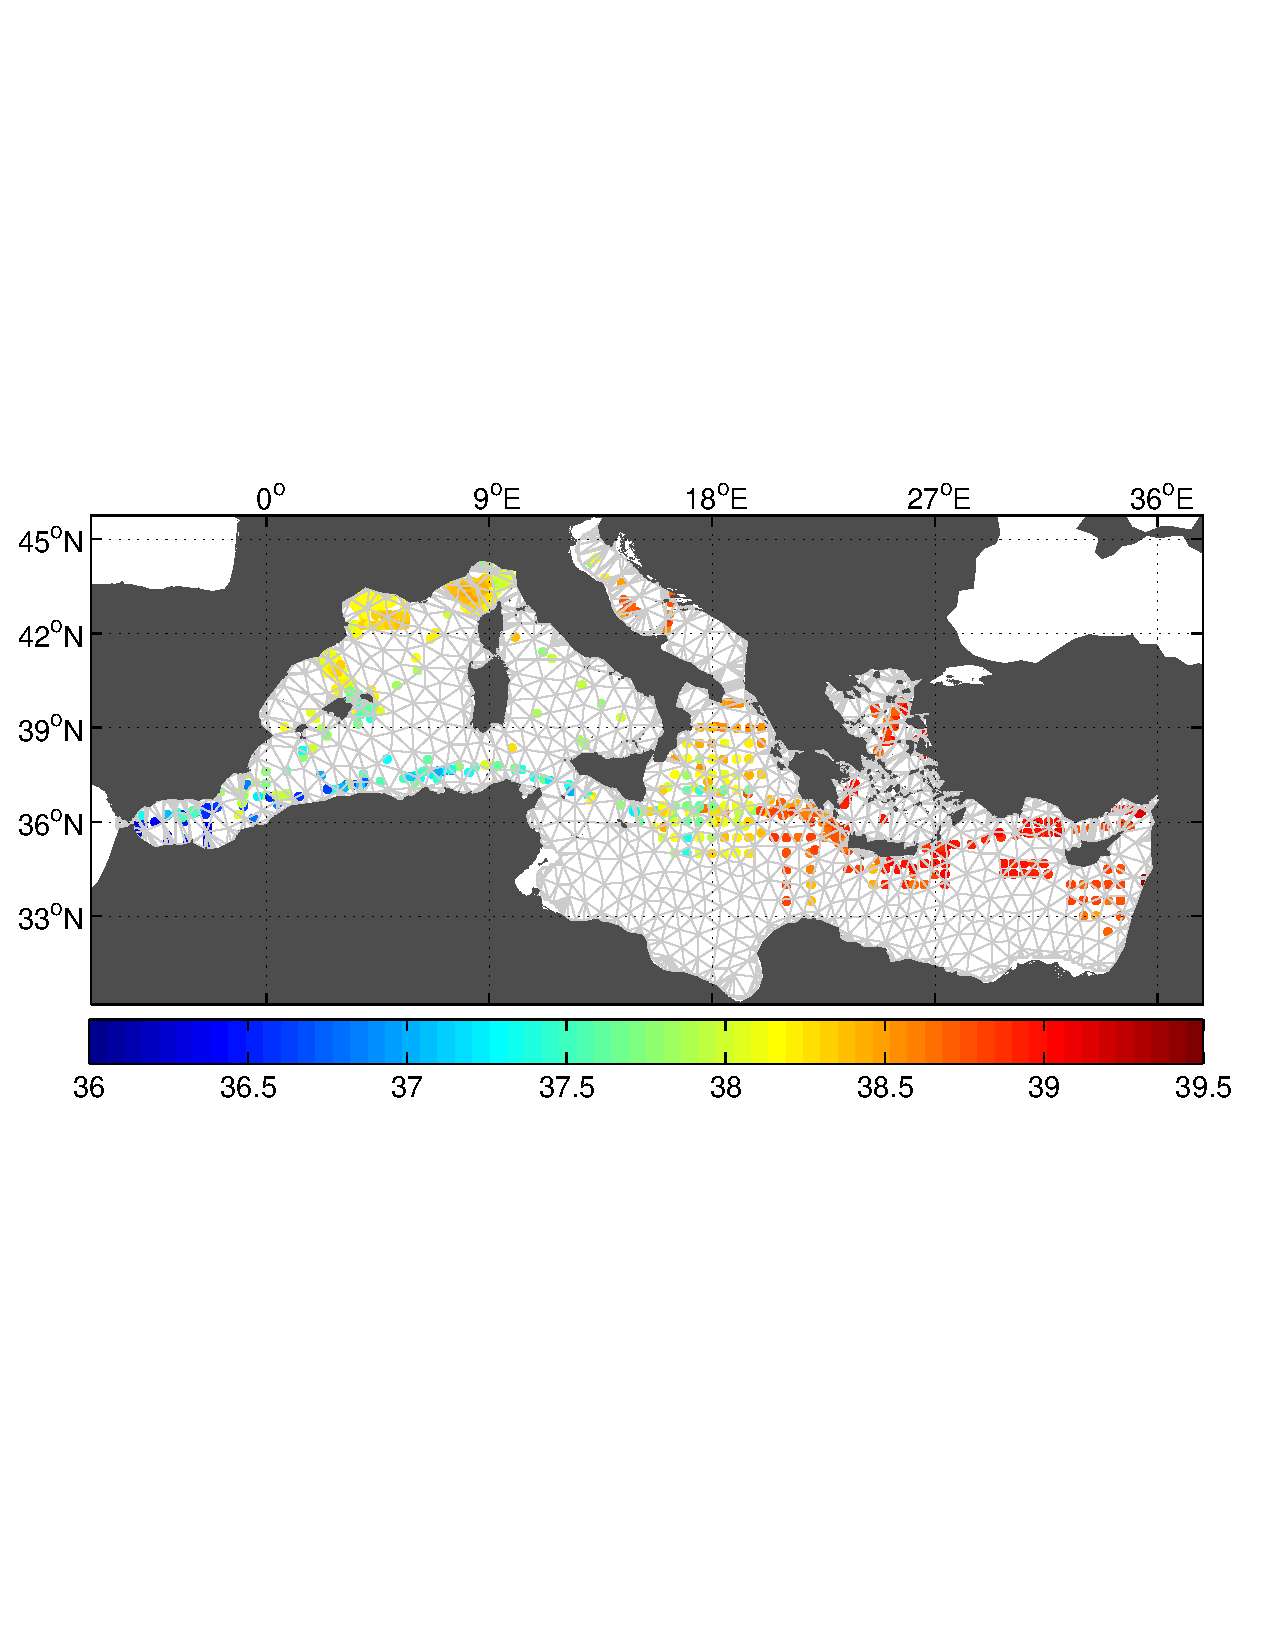
\includegraphics[width=.9\textwidth,bb=14 254 588 561]{diva_oi_09_10030dataval_mesh3}
\caption{Finite-element mesh and salinity measurements used for the application.\label{fig:diva_oi_09_10030dataval_mesh3}}
\end{figure}



\subsection{Parameters determination}
%------------------------------

\subsubsection{Correlation length}
%---------------------------------

\index{Correlation length}

The toold \command{divafit} will provide a first guess of the parameters $\snr$ and $L$. It will generates the output files:
\begin{description}
\item[\file{covariance.dat}:] contains distances between points, the covariance and the number of data couples used to estimate the covariance.
\item[\file{covariancefit.dat}:] contains the distance between points, the data-covariance and the fitted covariance.
\item[\file{paramfit.dat}:] contains estimates for the correlation length $L$ and for the signal-to-noise ratio $\snr$. You can manually replace the old values of $\snr$ and $L$ in \file{param.par} by the new ones from \file{paramfit.dat}.
\end{description}

If you want the new $L$ value to be automatically replaced, type 

\begin{lstlisting}[style=Bash]
bash-3.2$ divafit -r
\end{lstlisting}
%$

\begin{exfile}[H]
\begin{footnotesize}
\begin{verbatim}
Correlation length
   1.3565110
 Signal to noise ratio
  0.72524220
 VARBAK
  4.59391139E-02
 Quality of the fit (0: bad 1: good)
  0.85546345970344528
 For information: correlation length in km is   151.44691
\end{verbatim}
\end{footnotesize}
\caption{\file{paramfit.dat}}
\end{exfile}


The fit yields the value $L=1.36^{\circ}$ ($\simeq$ 151~km).

\begin{figure}[h!]
\centering
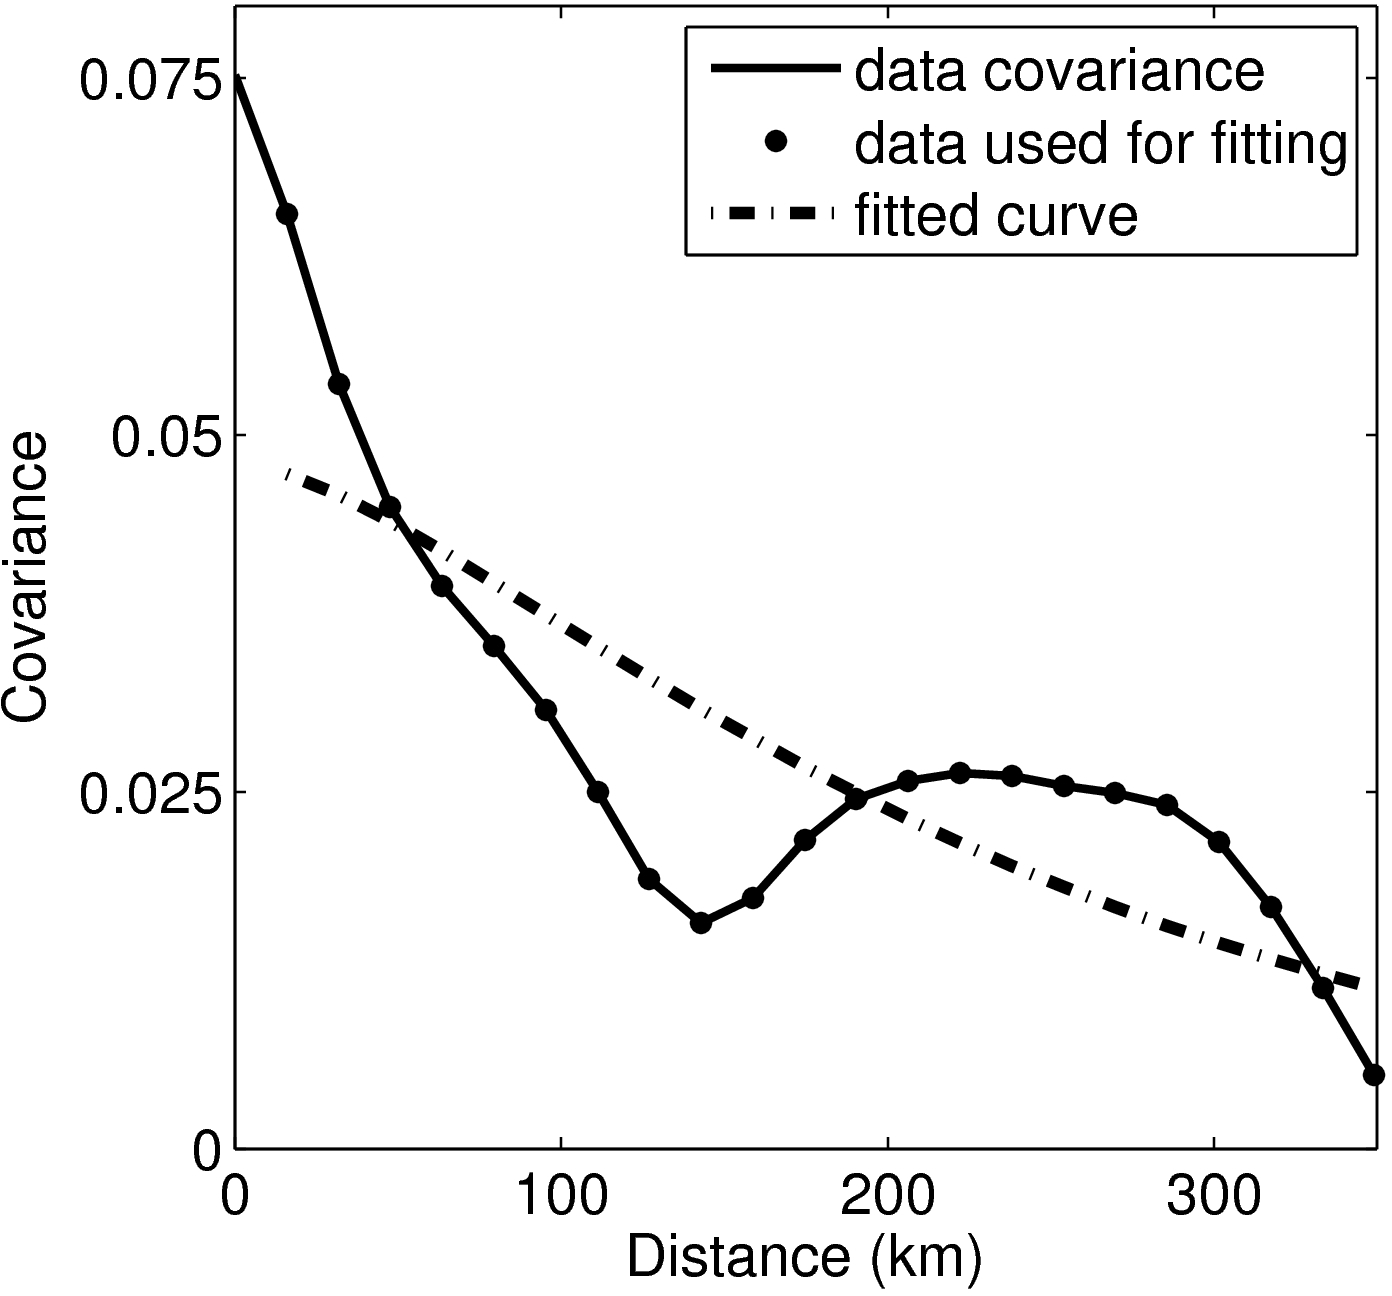
\includegraphics[width=.475\textwidth,bb=106 253 450 575]{Salinity_19502010_0707_10029e_fit}
\caption[Fit of the data correlation to the theoretical kernel.]{Fit of the data correlation to the theoretical kernel (dashed line). \label{fig:Salinity_19502010_0707_10029e_fit}}
\end{figure}



\subsection[Contour checking]{Contour checking (optional)}
%--------------------------------

If you want to check the contour file you want to use to generate the mesh, type \command{divacck}. The output \file{coast.cont.checked} is a thinned contour based on the length scale.
Then simply copy the new contour into the \directory{input} directory:

\begin{lstlisting}[style=Bash]
bash-3.2$ cp ./output/coast.cont.checked ./input/contour.cont
\end{lstlisting}

%$

\subsection{Mesh creation}
%------------------------------

\index{Mesh}
Simply type \command{divamesh} to perform the mesh generation. All the parameters needed by \diva are contained in \file{coast.cont}, \file{param.par} and \file{coast.cont.dens} if you work with a non-uniform mesh.
The mesh corresponding to this example is shown in Fig.~\ref{fig:diva_oi_09_10030dataval_mesh3}. For the sake of visibility, the mesh was generated with a rather long characteristic scale: the correlation length was set to $3^{\circ}$, meaning the typical length of triangle edge is about 1$^{\circ}$


\subsection{Generalised Cross Validation}
%-------------------------------------

\index{Generalised cross validation}
GCV provides you with improved estimates of parameters (see Chapter~\ref{chap:analysisparameters} for a detailed description of the method). You need to provide an input file \file{gvcsampling.dat} (see example file \ref{gcvsampling}) containing a list of values for the signal-to-noise ratio on which you want to try the estimator.

Type \command{divagcv} to perform the GCV on these values. Optimal values for the parameters are given in \file{gcvsnvar.dat} (example file \ref{gcvsnvar}). You can then modify \file{param.par} (example file \ref{paramfileCL2}) according to these values before performing an analysis. 

\begin{exfile}[H]
\begin{footnotesize}
\begin{verbatim}
0.1
0.5
1
5
10
50
100
\end{verbatim}
\end{footnotesize}
\caption{\file{gvcsampling.dat}. \label{gcvsampling}}
\end{exfile}


\begin{exfile}[H]
\begin{footnotesize}
\begin{verbatim}
  S/N , VARBAK
  68.7858658   2.05896711
\end{verbatim}
\end{footnotesize}
\caption{\file{gcvsnvar.dat}. \label{gcvsnvar}}
\end{exfile}



\begin{exfile}[htpb]
\begin{footnotesize}
\begin{verbatim}
# Lc: correlation length (in units coherent with your data)
2.76536822
# icoordchange (=0 if no change of coordinates is to be performed; 
=1 if positions are in degrees and if you want to use real distances)
1
# ispec (output files required, comments to come)
3
# ireg (mode selected for background field: 0=null guess; 1=mean of data; 
2=regression plan if at least 3 non-aligned data provided)
1
# xori: x-coordinate of the first grid point of the output
-10.0
# yori: y-coordinate of the first grid point of the output
30
# dx: step of output grid
0.2
# dy: step of output grid
0.2
# nx: number of grid points in the x-direction
236
# ny: number of grid points in the y-direction
81
# valex: exclusion value
-9999.0
# snr: signal to noise ratio of the whole data set
68.7858658   
# varbak variance of the background field. 
If zero, no error fields are produced. If one, relative errors are obtained
2.05896711
\end{verbatim}
\end{footnotesize}
\caption{Adapted version of \file{param.par}\label{paramfileCL2}}
\end{exfile}

\subsection{Analysis}
%-----------------

\diva analysis is executed by typing \command{divacalc}. It not only provides the analysed field, but also the error field if $\texttt{varbak}$ is not equal to zero. Results are presented in Figs.~\ref{analysisCL1} and \ref{analysisCL1}.

\begin{figure}[htpb]
\centering
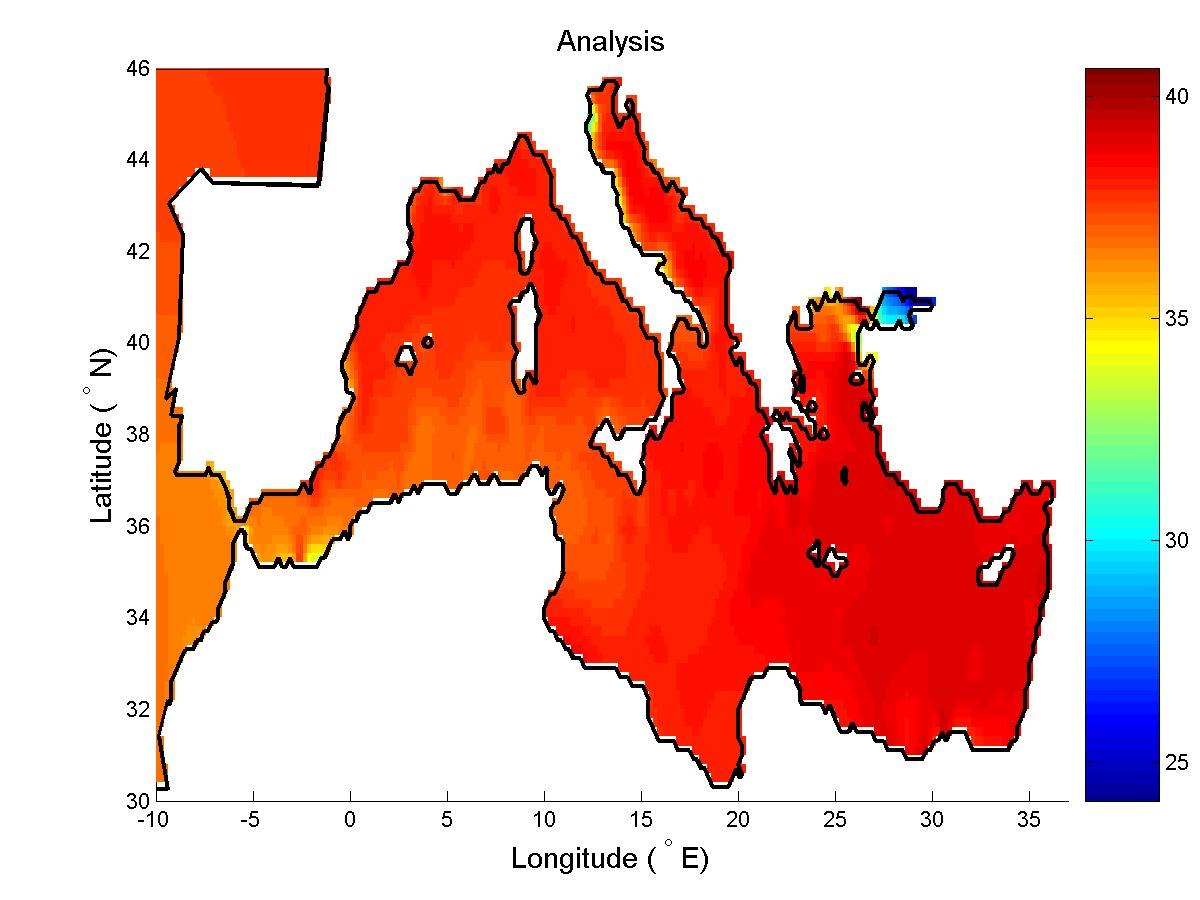
\includegraphics[width=.75\textwidth]{medar_analysis}
\caption{Analysed salinity field with the parameters from \command{divagcv}.\label{analysisCL1}}
\end{figure}


\begin{figure}[htpb]
\centering
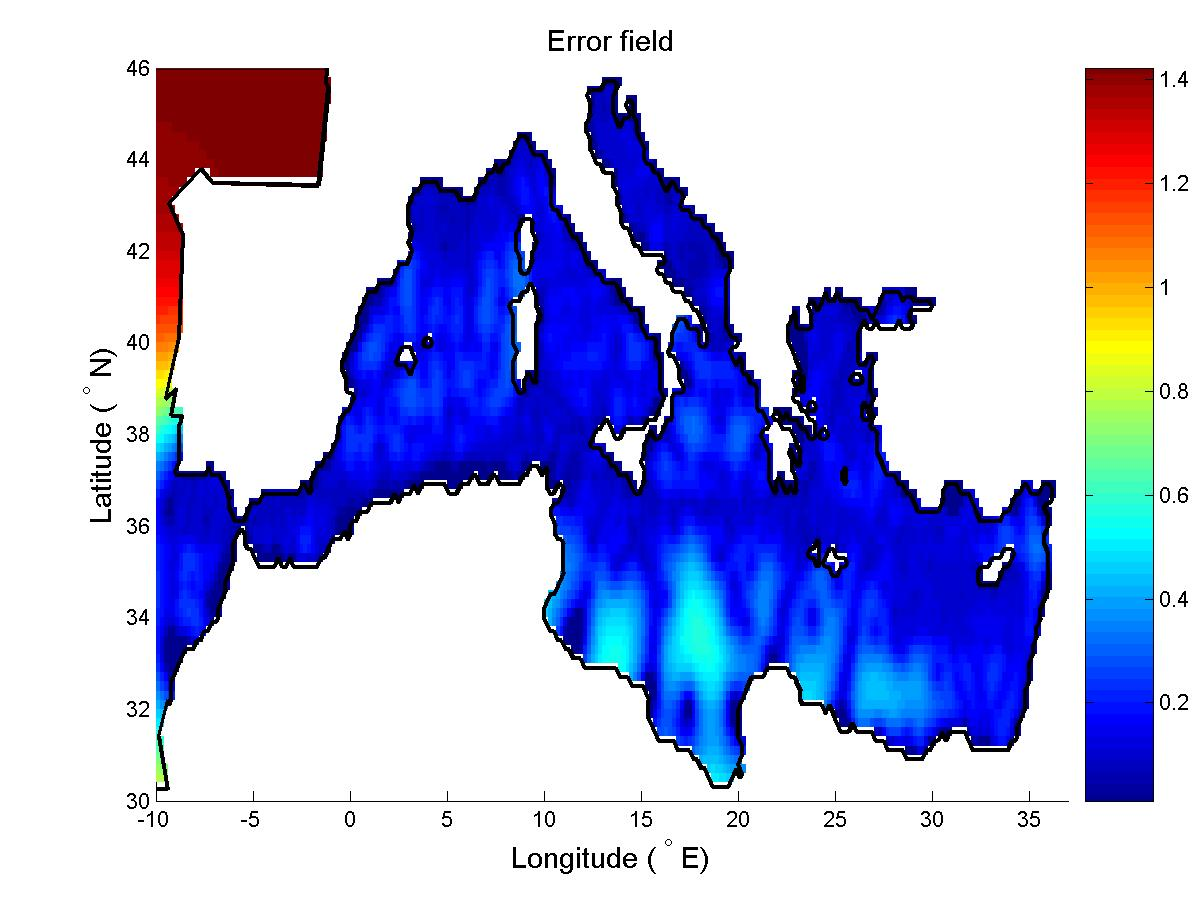
\includegraphics[width=.75\textwidth]{medar_error}
\caption{Error field and data locations with the parameters from \command{divagcv}.\label{errorCL1}}
\end{figure}



\clearpage
%\subsection{Quality control}
%%%------------------------
%
%Three \diva modules are dedicated to quality control and detection of outliers. Criteria to detect outliers are presented in Sec. \ref{secdivaqc}. We tried the three modules on our dataset with the parameters taken from file \ref{paramfileCL2}.


%\begin{figure}[H]
%\centering
%\includegraphics[width=.75\textwidth]{medar_divaqc}
%\caption{Example of output generated by \texttt{divaqc} using the parameters from \texttt{divagcv}.\label{divaqcCL}}
%\end{figure}


%\begin{figure}[H]
%\centering
%\includegraphics[width=.75\textwidth]{medar_divaqcbis}
%\caption{Example of output generated by \texttt{divaqcbis} using the parameters from \texttt{divagcv}.\label{divaqcbisCL}}
%\end{figure}
%
%
%\begin{figure}[H]
%\centering
%\includegraphics[width=.75\textwidth]{medar_divaqcter}
%\caption{Example of output generated by \texttt{divaqcter} using the parameters from \texttt{divagcv}.\label{divaqcterCL}}
%\end{figure}



%-----------------------------------------------------------------------------------------------------





\section{Analysis of profiles from a cruise\label{sec:cruise}}
%-----------------------------------------------------------------

Usually \diva is used in horizontal planes and the coordinate system deals with longitude and latitude. One may also want to use \diva for interpolating data obtained during a campaign, i.e., several profiles along a determinate trajectory. In this case, the user will work in vertical planes: $x-$coordinate will be a (curvilinear) distance and y-coordinate will be the depth.

In horizontal planes, domains are physically limited by coastlines, while in vertical planes, the boundaries will be the sea surface and the bottom. The domain will be closed by artificial vertical lines, for example lines that originate from the first and last stations of the cruise (Fig.~\ref{fig:data}(b)).

We present hereinafter a complete example for this type of interpolation.


\subsection{Creation of the contour}
%------------------------------------

Generally the contour generation is easier in this case, since the transect cannot cross islands. Let us consider a transect that follows the track presented on Fig.\ref{fig:data}. The first step is to extract topography, which acts as a boundary of our domain. Methods for getting a topography are detailed in Section~\ref{sec:howtotopo}. For the horizontal axes, we worked with the distance computed with respect to the starting position of the cruise. Other choices are possible, i.e., degrees of longitude or latitude, distance from a reference point\ldots

\begin{figure}[htpb]
\centering
\subfigure[Localization of the data (triangles) and topography of the region]{
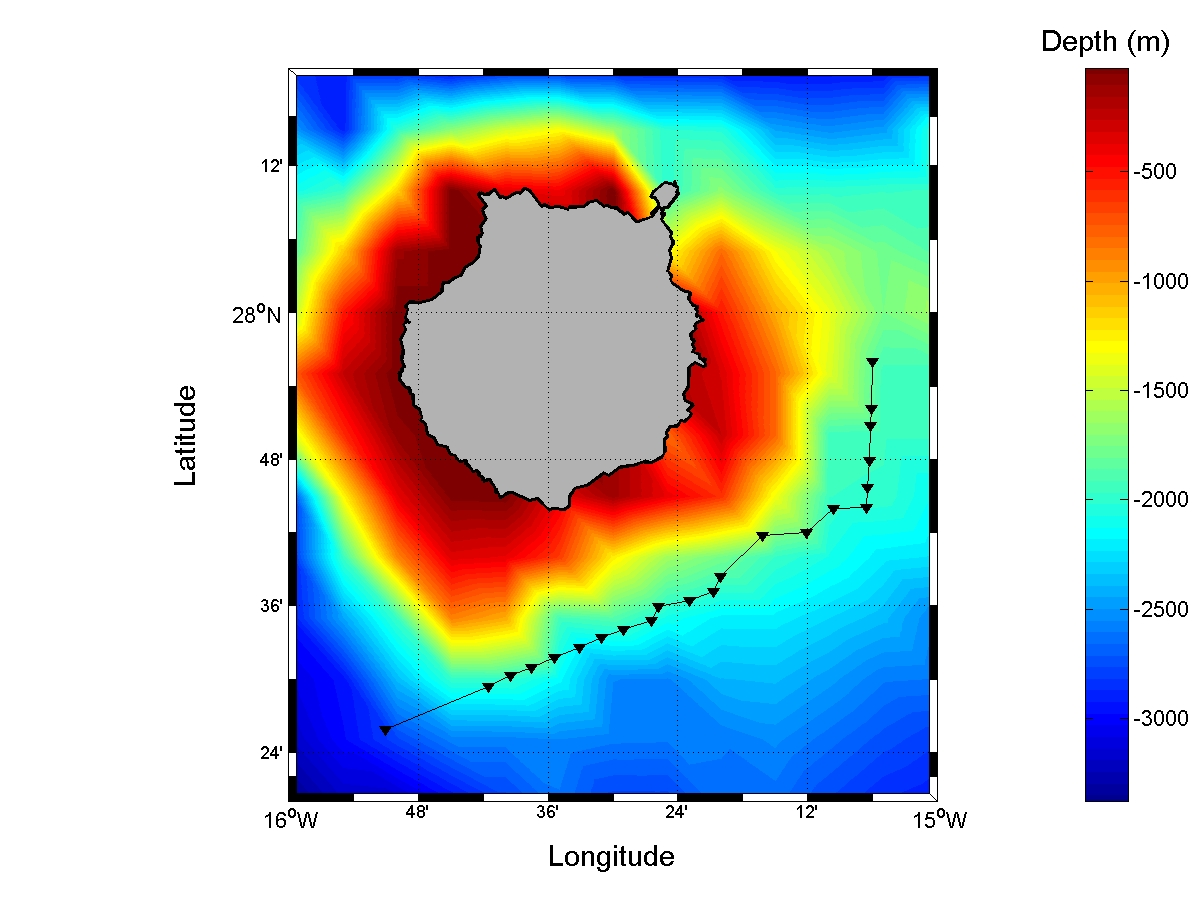
\includegraphics[width=.475\textwidth]{cruise_profiles}
}\subfigure[Data with limits of the domain]{
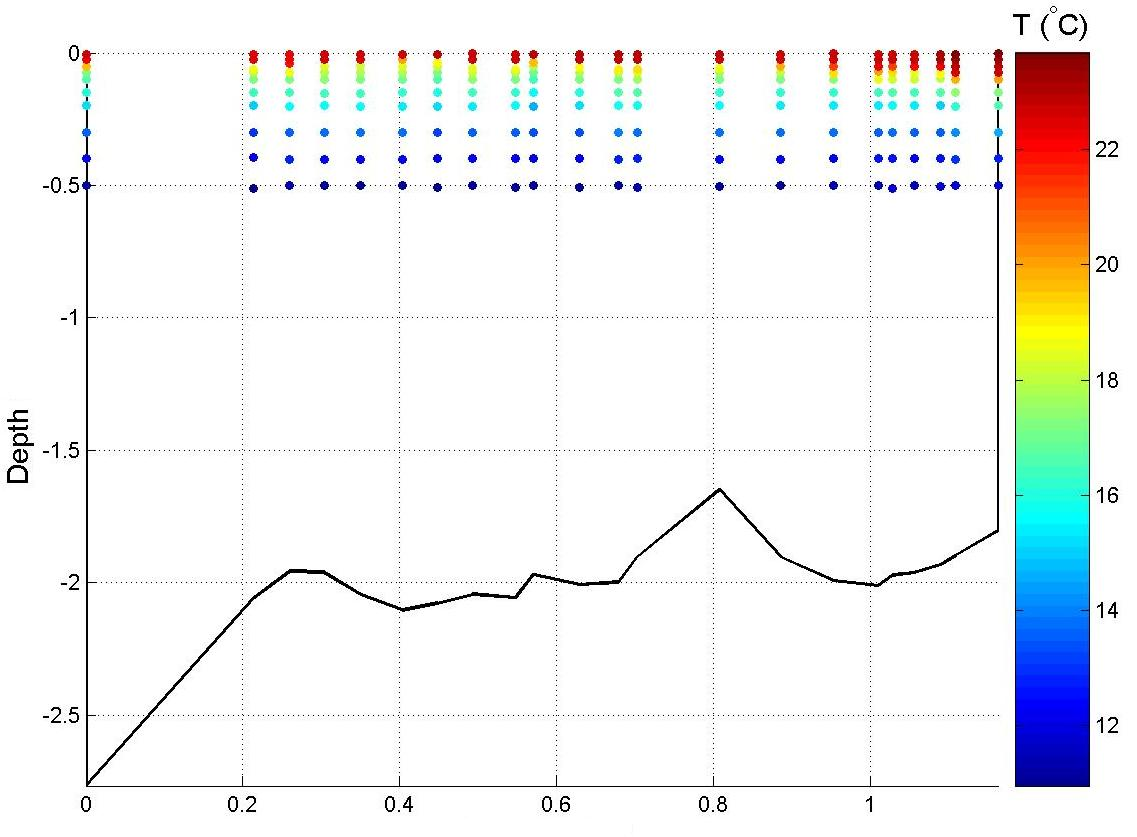
\includegraphics[width=.475\textwidth]{cruise_data_contour}
}
\caption{Contour generation.\label{fig:data}}
\end{figure}


\begin{exfile}
\begin{footnotesize}
\begin{verbatim}
1 
24 
0.000000 0.000000 
0.000000 -2.766513 
0.213350 -2.058027 
0.259753 -1.956031 
0.303870 -1.960115 
0.350149 -2.044557 
...
1.108852 -1.895979 
1.162687 -1.804136 
1.162687 0.000000 

\end{verbatim}
\end{footnotesize}
\caption{Contour file of Fig.~\ref{fig:data}(b).\label{exfile:contour}}
\end{exfile}


\subsection{Mesh generation\label{sec:meshscale}}
%------------------------------------------------

%As a first try we want to work with the correlation length provided by the tool \texttt{divafit}, but the tool is not able to provide us with a value of the correlation length because of the difference in length scales.


\index{Mesh}
Since in physical oceanography, vertical length scales (100-1000\,m) are much smaller than horizontal length scales (100-1000\,km), an improvement is  made if we take into account this anisotropy. To this end we need estimates of $L_{x}$ and $L_{y}$, the horizontal and vertical length scales, respectively.


The most direct solution is to compute, for $L_{x}$, the mean distance between two stations, and for $L_{y}$, the mean distance between two measurements on a same profile. Then we compute the ratio

\[r = \frac{L_y}{L_x}\]

and multiply the horizontal coordinates by $r$. This allows one to work with the same length scale both on vertical and horizontal directions. With the  data set from Fig.~\ref{fig:data}(b), we obtain:

\begin{eqnarray*}
L_{x} &=& 4.4\,km,\\
L_{y} &=& 55\,m,\\
	r   &=& 0.0125.
\end{eqnarray*}

We then compute the length scale with the help of \command{divafit} and generate a new mesh, showed on Fig.~\ref{fig:mesh}. 

\begin{figure}[H]
\centering
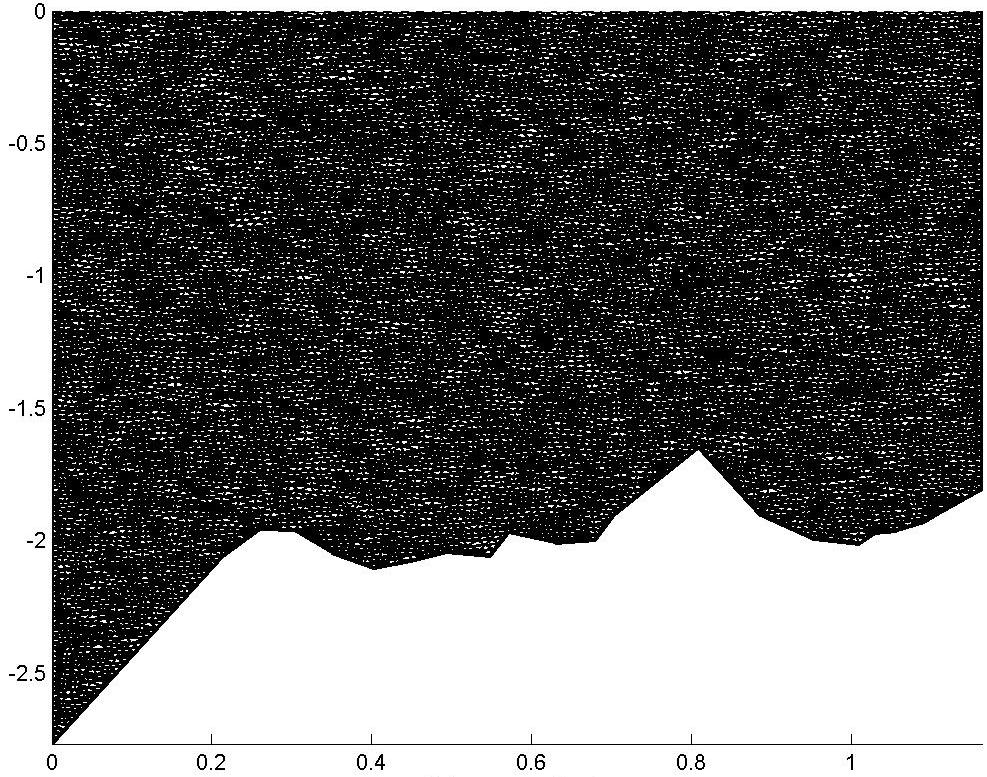
\includegraphics[width=.475\textwidth]{cruise_mesh}
\caption{Mesh generated in the scaled domain.\label{fig:mesh}}
\end{figure}

\subsubsection{Use of negative \texttt{icoordchange}}
%-------------------------------------------

A more direct way to do the previous operation consists in changing the value of \texttt{icoord\-change} in file \file{param.par}: by assigning a negative value to this parameter, we apply a scaling on the $x$ coordinate (Sec.~\ref{sec:icoord}). In the present case we would put\, \texttt{icoordchange = -0.0125}. Then the classical \diva operations can be done.



\subsection{Analysis}
%--------------------

Once the mesh is created, the analysis is straightforward. The only thing to be aware of is the specification of the domain in file \file{param.par}: as we worked with scaled coordinates when generating the mesh, we have to do the same when specifying \texttt{x/yorigin} and \texttt{dx/y}. After the analysis, we may simply multiply the $x$ coordinate by $r$ to recover the original values. The results are presented on Fig.~\ref{fig:analysis}.  

 
\begin{figure}[htpb]
\centering
\subfigure[Reconstructed temperature field]{
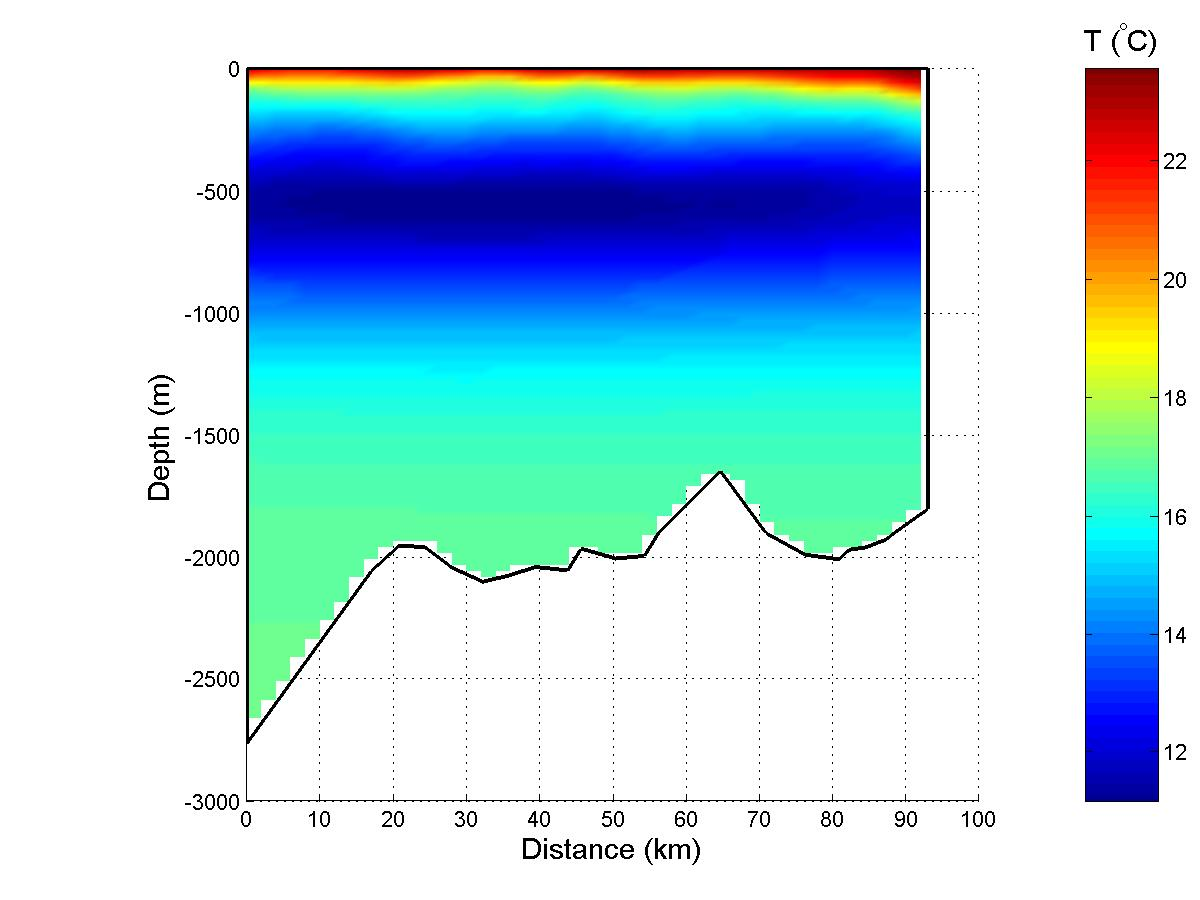
\includegraphics[width=.475\textwidth]{cruise_analysis}
}\subfigure[Zoom between 0 and 500 m]{
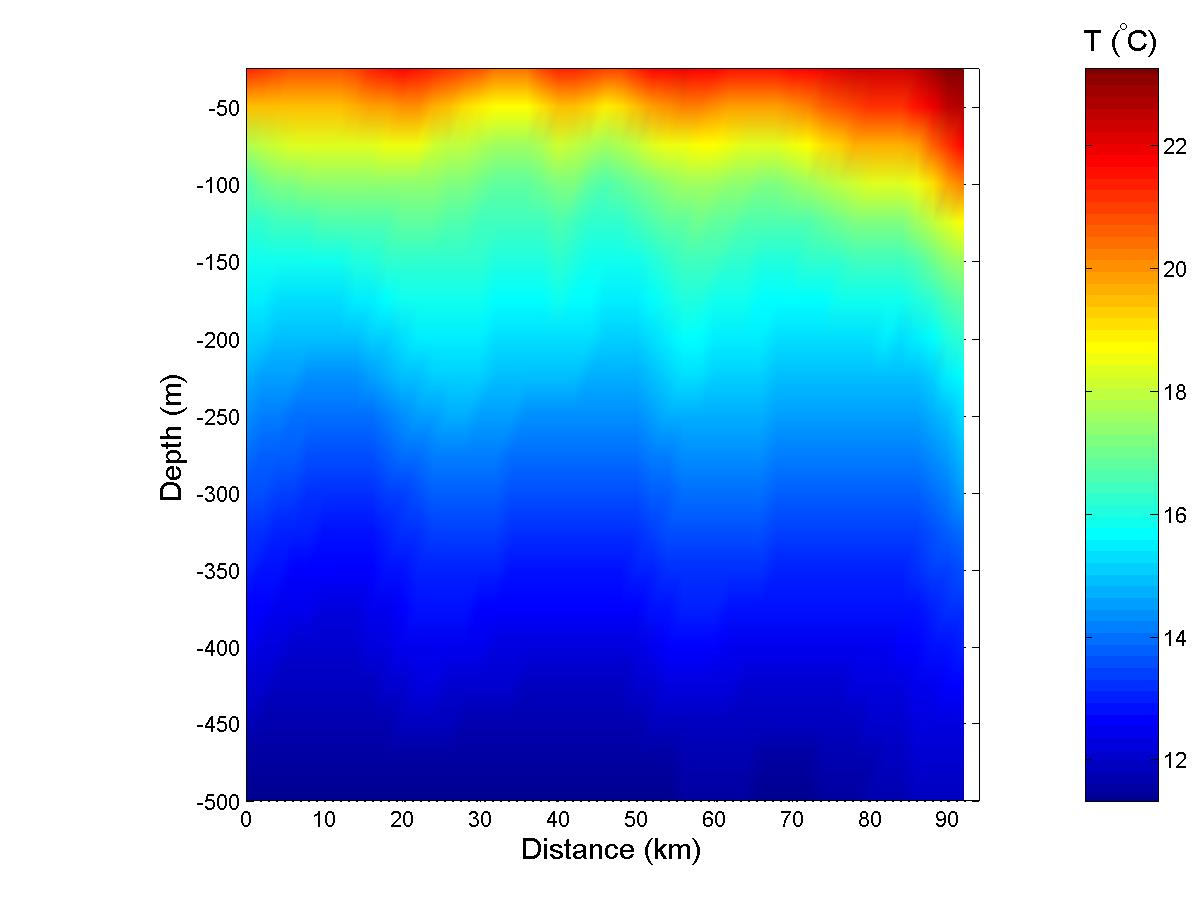
\includegraphics[width=.475\textwidth]{cruise_analysis_zoom}
}
\caption{Results of analysis.\label{fig:analysis}}
\end{figure}





\section{Analysis of data from a transect}
%-------------------------------------------------

This case is very similar to the previous one. the difference is that here, data are collected along a trajectory of constant latitude.
\subsection{Data}
%-------------

The track of the cruise (Fig.~\ref{fig:transectprofiles}) follows a trajectory of constant latitude (24$^{\circ}$ N) across the Atlantic Ocean. Salinity for the year 1958 is represented on Fig.~\ref{fig:domaindata} along with the topography. 

\begin{figure}[htpb]
\centering
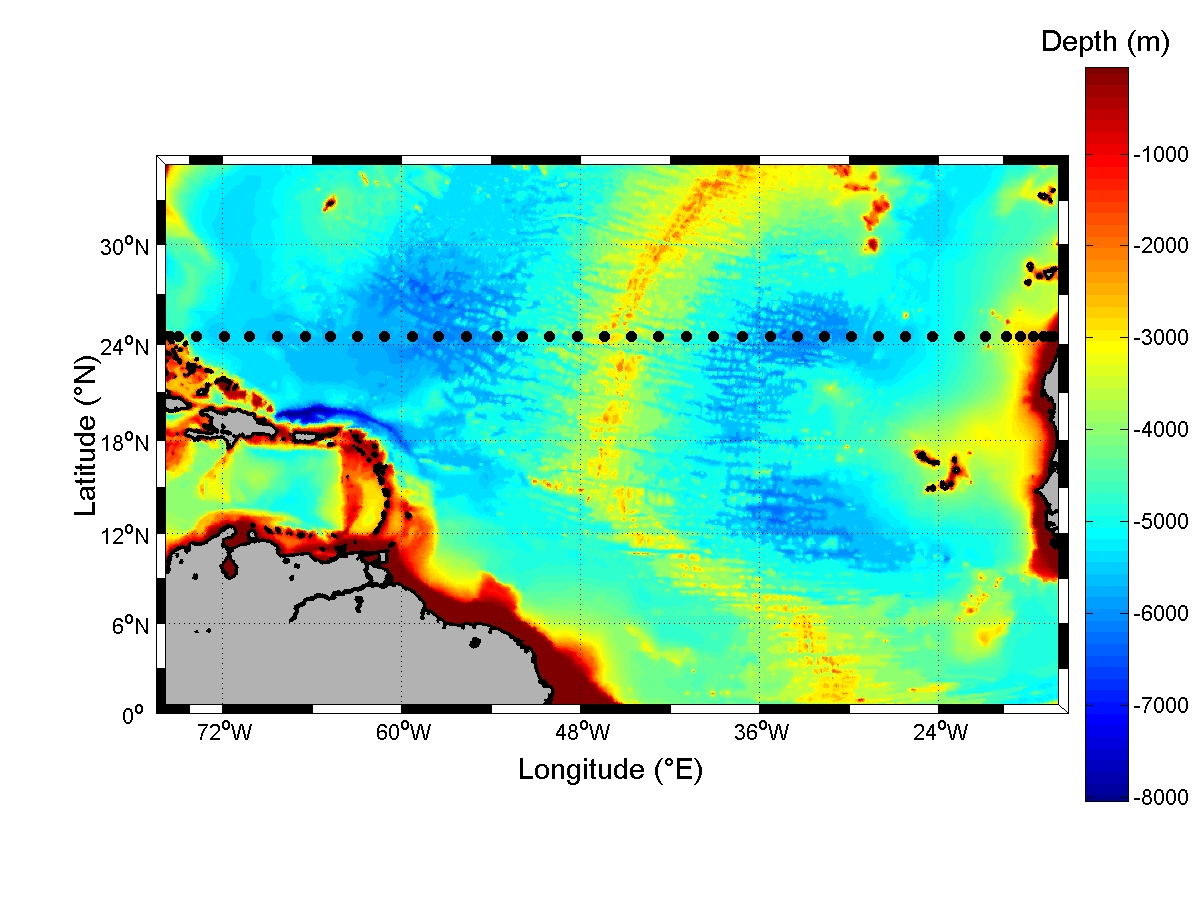
\includegraphics[width=.75\textwidth]{TransAtlant_stations}
\caption{Transect stations ($\bullet$) and bottom topography.\label{fig:transectprofiles}}
\end{figure}

\subsection{Contour creation}
%-------------------------

We have to convert degrees of longitude into kilometres to be coherent with the units, since the depth cannot be expressed in degrees. To this end, we used \matlab function \file{distance.m}, which calculates the \textit{great circle distances} between two points on the surface of a sphere.  

\subsubsection{Extraction of topography}
%------------------------------------

We extract topography with the help of \matlab function  \file{m\_tbase.m}, which uses $5-$minute TerrainBase database. But any other source of topography suits.
				
\begin{figure}[H]
\centering
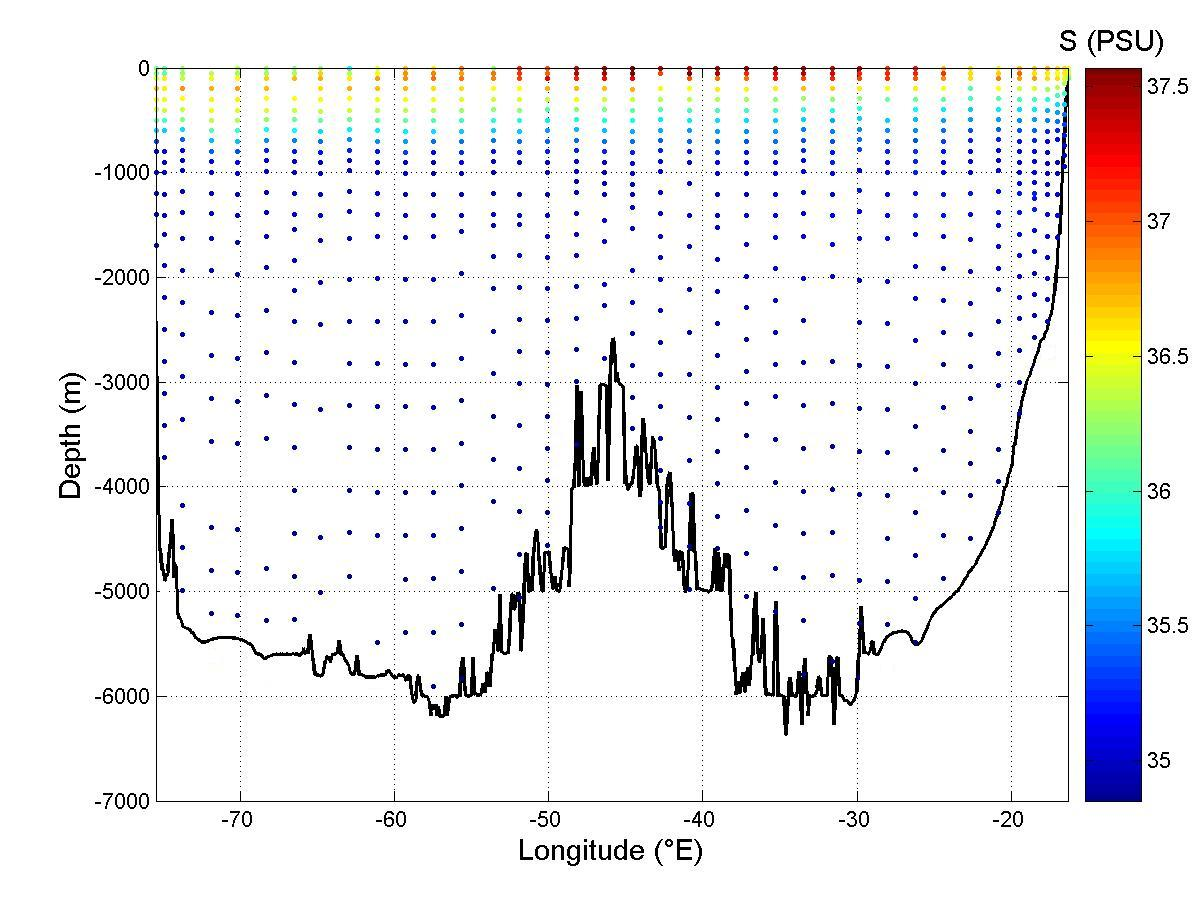
\includegraphics[width=.75\textwidth]{TransAtlant_data_contour2}
\caption{Domain and data.\label{fig:domaindata}}
\end{figure}


%\subsubsection{Contour check}
%%-------------------------
%
%\diva tool \command{divacck} allows us to be sure we do not have any crossing or any identical points in the domain. 
%

\subsection{Mesh} 
%----------------

\subsubsection{Computation of length scales}
%----------------------------------------

Similarly to the previous case, we compute horizontal and vertical length scales in order to take into account the domain anisotropy. Fig.~\ref{fig:anisotropy} illustrates the difference between horizontal and vertical scales, as we represented the data within the domain with axes graduated in kilometres.

For $L_x$ and $L_y$, the same definitions as in Section~\ref{sec:meshscale} are used. We find

\beqn
L_x &=& 156.76\,km, \\
L_y &=& 204.40\,m, \\
\textrm{and the ratio\qquad} r &=&  0.0013.
\eeqn

\begin{figure}[htpb]
\centering
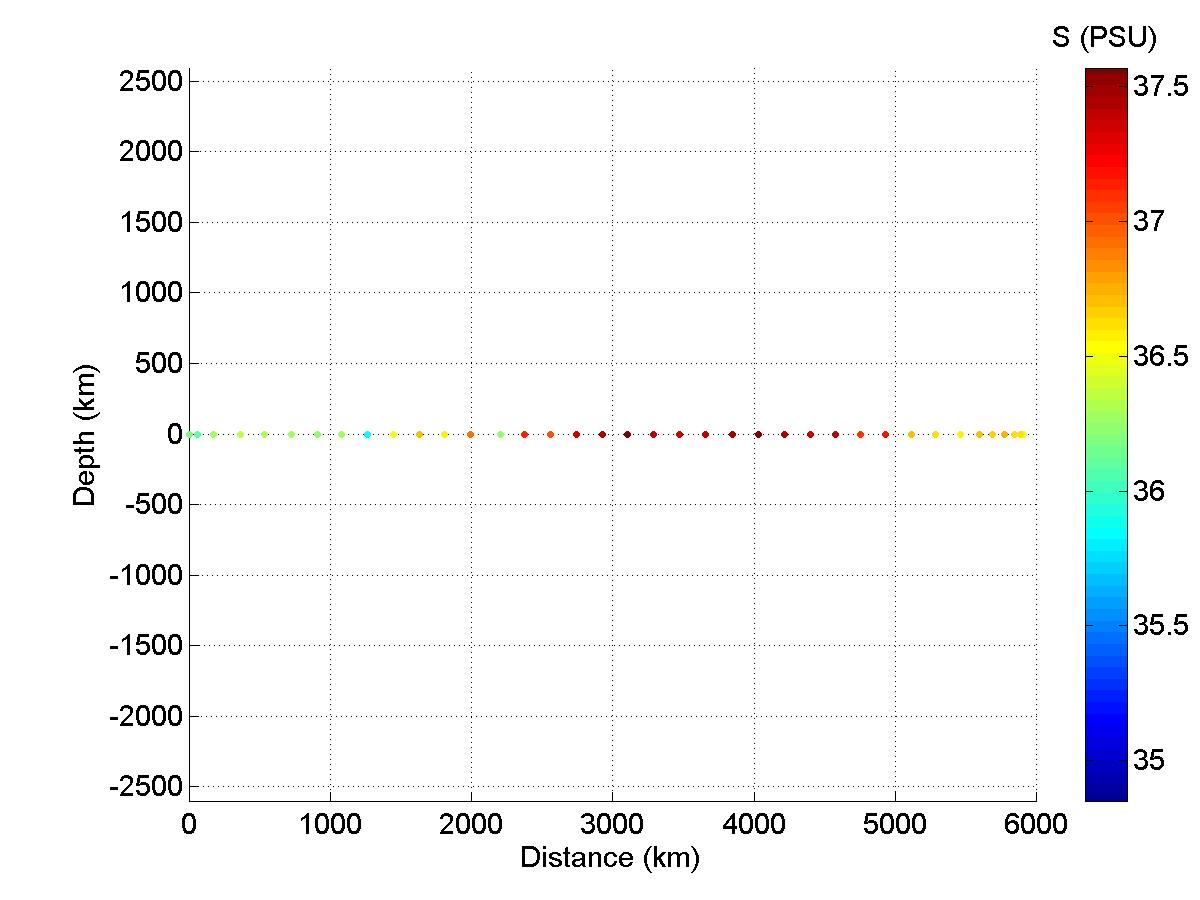
\includegraphics[width=.75\textwidth]{anisotropy}
\caption{Data with axes in kilometres.\label{fig:anisotropy}}
\end{figure}



\subsubsection{Computation of correlation length}
%---------------------------------------------

\index{Correlation length}
Correlation length is estimated with the help of \command{divafit}, which gives us:

\[L=0.433\,km.\]

We generate the mesh (Fig.~\ref{fig:trans_mesh}) with this value.

\begin{figure}[H]
\centering
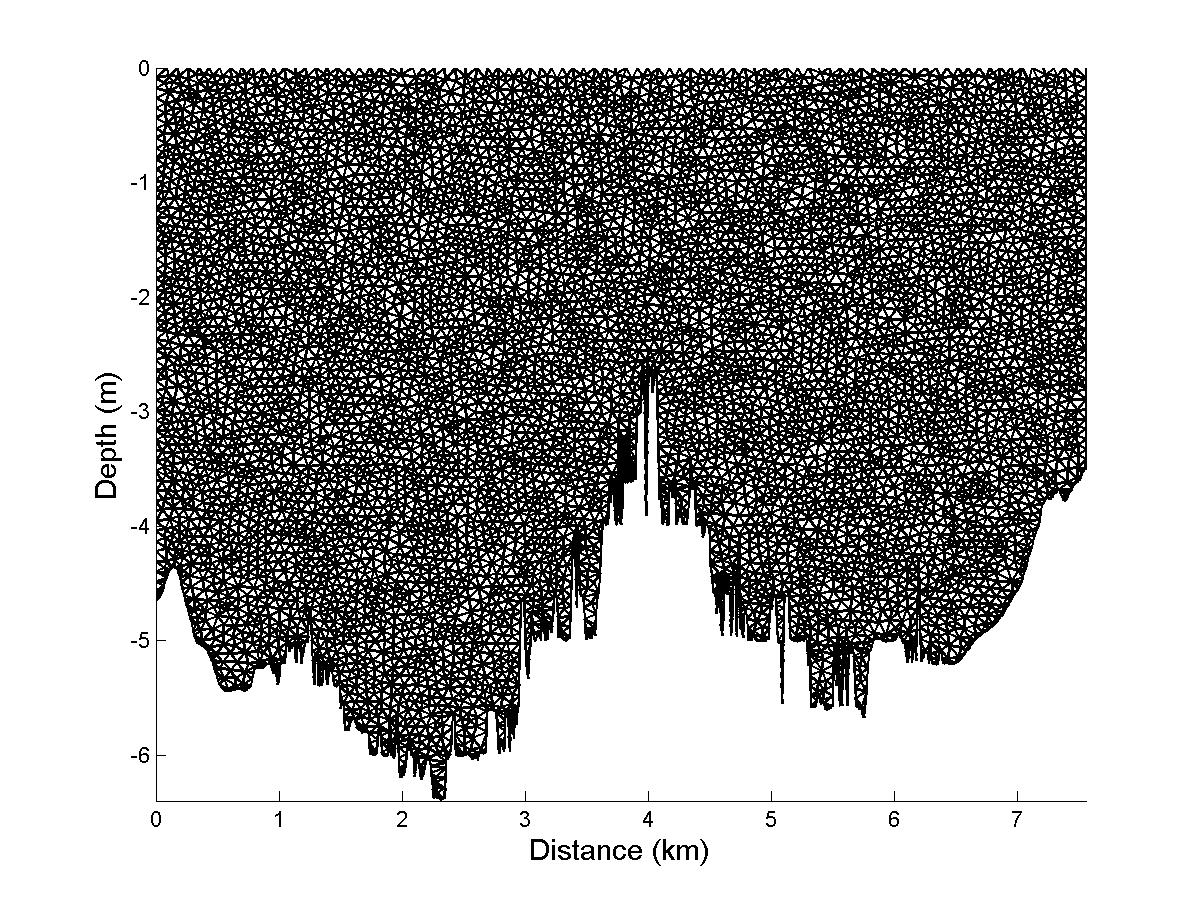
\includegraphics[width=.75\textwidth]{TransAtlant_mesh}
\caption{Mesh in the rescaled domain.\label{fig:trans_mesh}}
\end{figure}



\subsection{Analysis}
%-----------------

\subsubsection{Specification of the output grid}
%--------------------------------------------

%As the output grid is not regular, we will use file \texttt{valatxy.coord}. 
%to specify where we want the output. 

To be coherent with the scaling we made with the contour, we also have to consider scaled coordinates when specifying the output locations. 
Working in this coordinate system, we carry out an analysis with the following values (in kilometres):

\beqn
\texttt{xori} &=& 0\\
\texttt{yori} &=& -6.0\\
\texttt{dx} &=& 0.01\\
\texttt{dy} &=& 0.002,\\
\eeqn

which gives us a  $809\, \times\, 299$ point grid. Results are presented on Figs.~\ref{fig:transectanalysis} and \ref{fig:transanalysiszoom}

\begin{figure}[H]
\centering
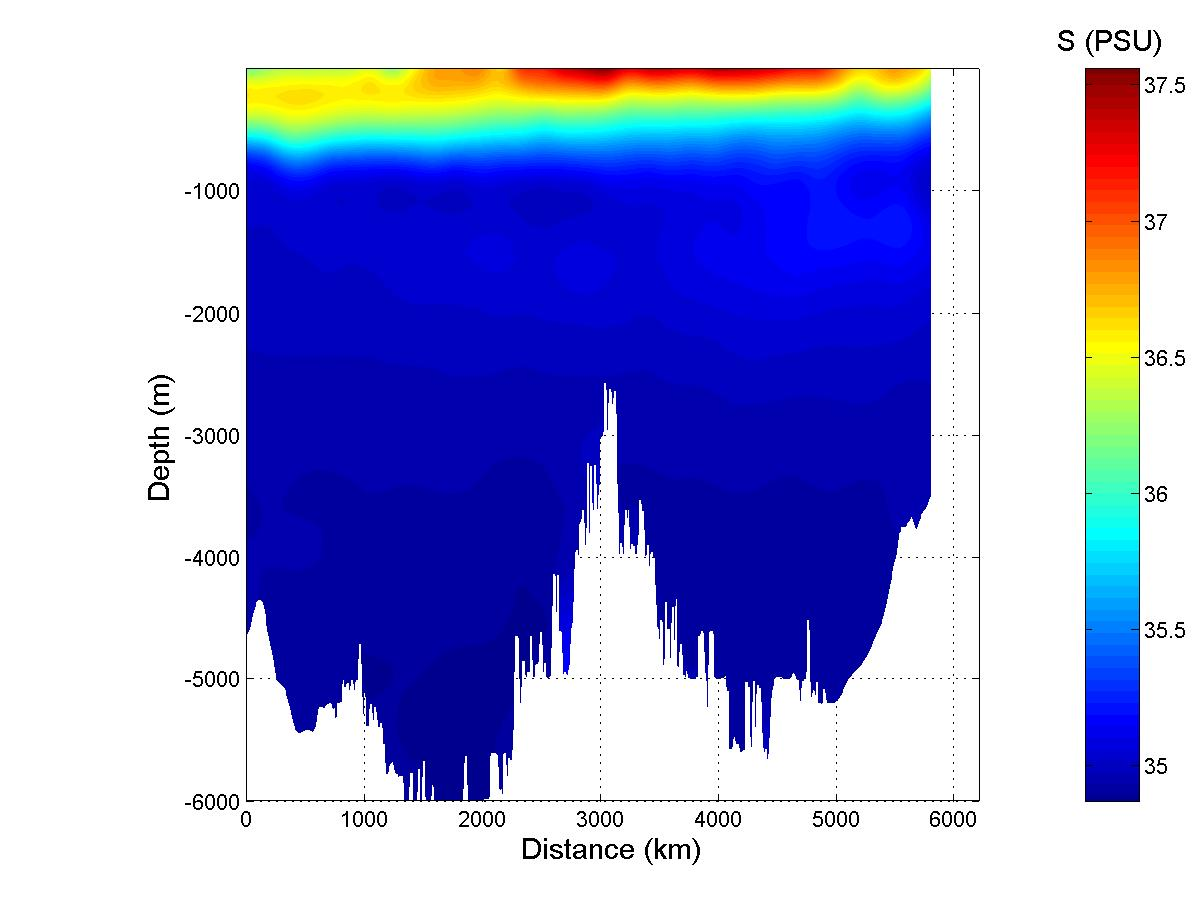
\includegraphics[width=.75\textwidth]{TransAtlant_analysis2}
\caption{Analysed field.\label{fig:transectanalysis}}
\end{figure}


\begin{figure}[H]
\centering
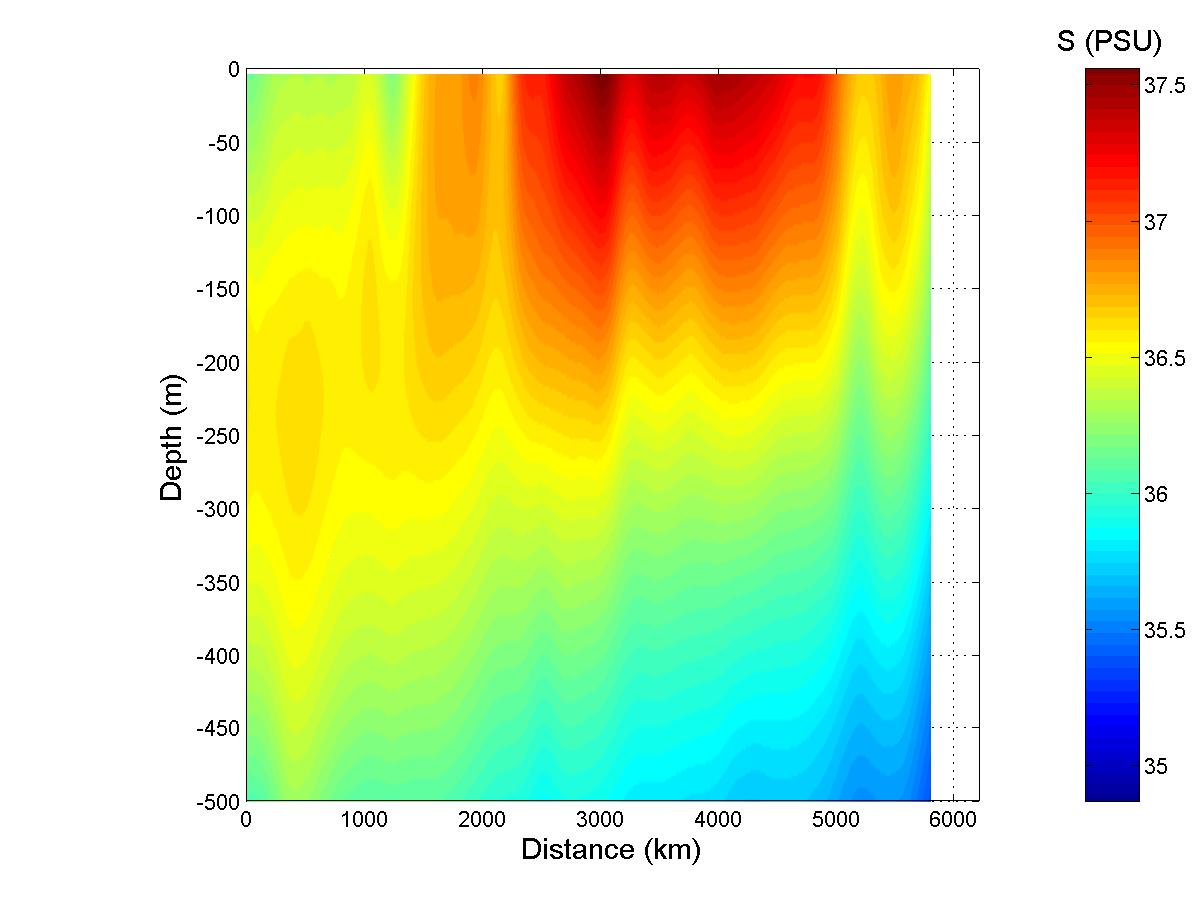
\includegraphics[width=.75\textwidth]{TransAtlant_analysis_zoom2}
\caption{Analysed field between 500 m and sea surface.\label{fig:transanalysiszoom}}
\end{figure}




\section[Advection constraint]{Advection constraint: Mediterranean Sea}
%-----------------------------------------


\index{Advection}
In this example, data points are located on a regular grid with alternate values of $-1$ and $+1$. An analysis with isotropic OI \index{OI} yields the field shown in Fig.~\ref{fig:medregiso}: we obtain a pattern of alternating circular isolines on the whole domain (land is treated as it was sea). The analysis with \diva shows the influence of coastlines, as differences between the two cases are more obvious near coasts (Fig.~\ref{fig:medregtopo}).  

\begin{figure}[H]
\centering
\parbox{.6\textwidth}{
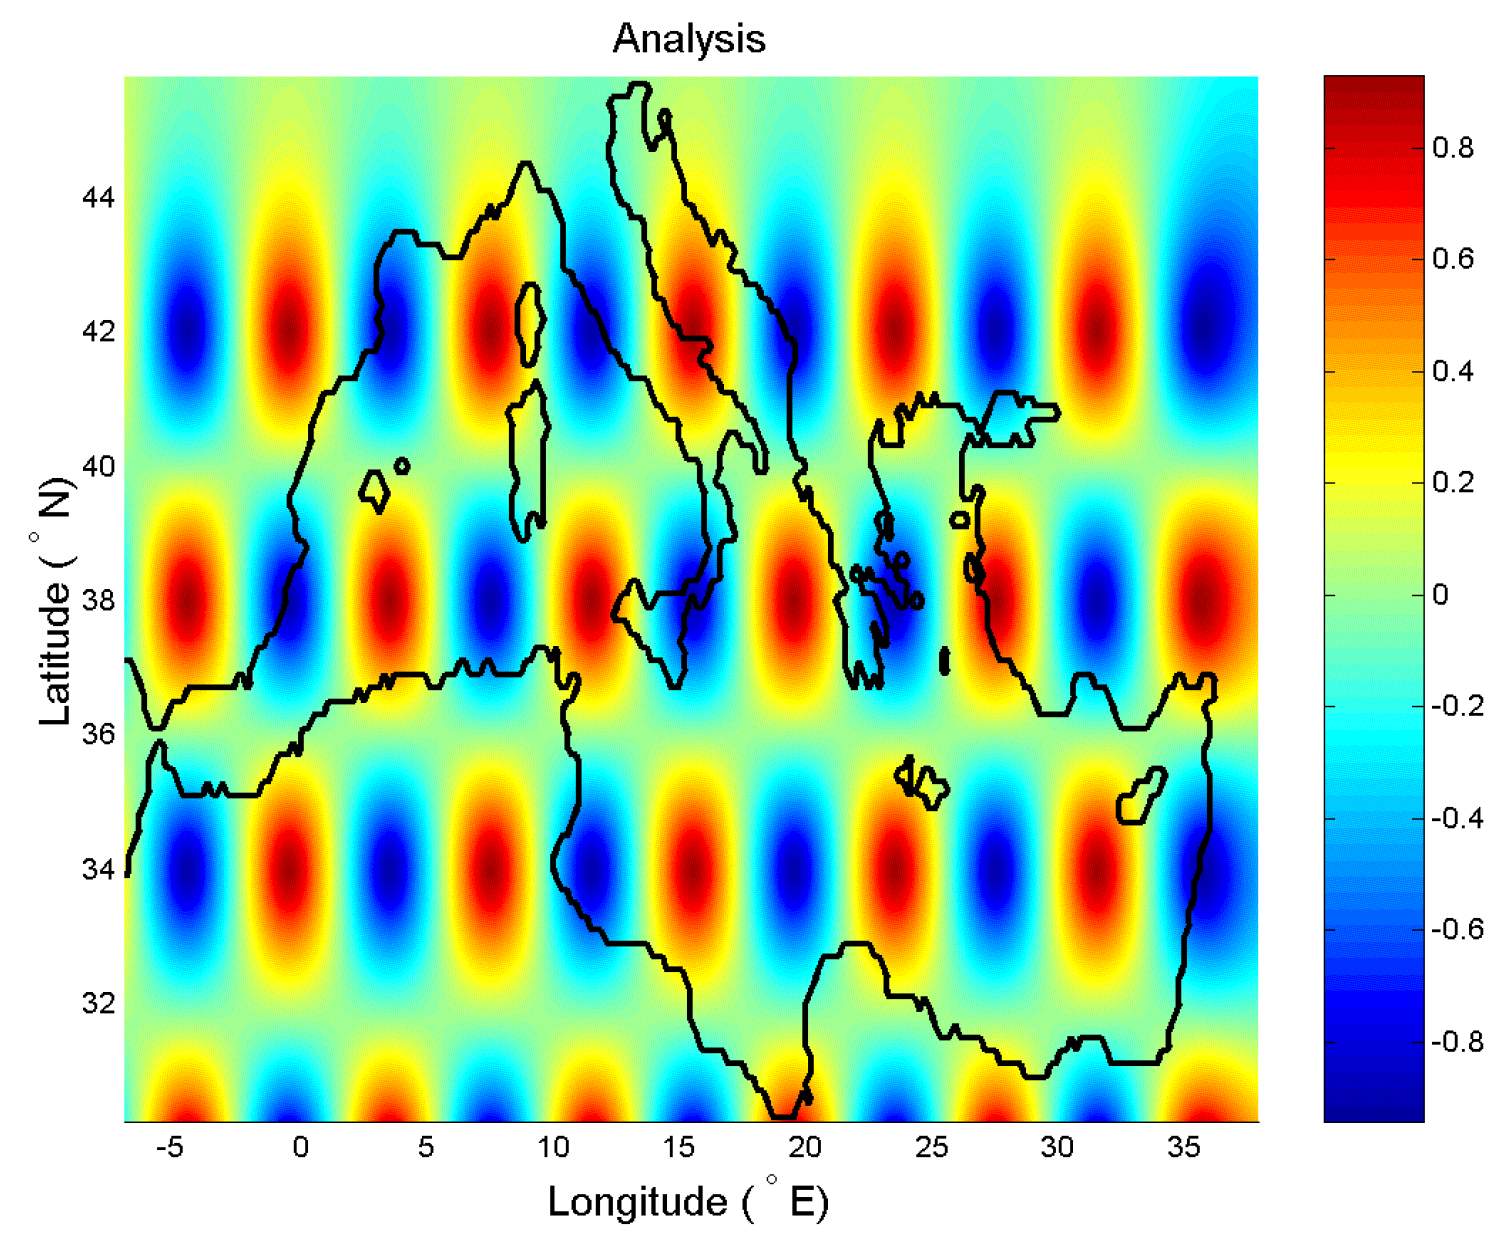
\includegraphics[width=.55\textwidth]{medregiso}
}\parbox{.4\textwidth}{
\caption{Isotropic OI.\label{fig:medregiso}}
}
\end{figure}


\begin{figure}[H]
\centering
\parbox{.6\textwidth}{
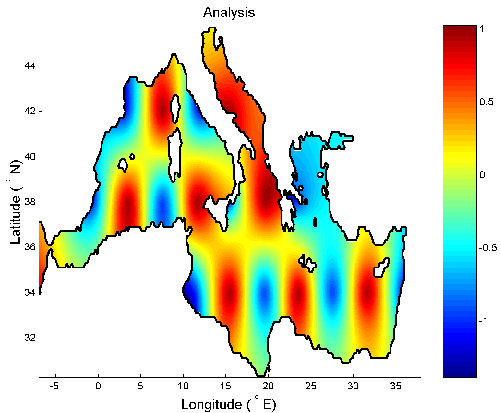
\includegraphics[width=.55\textwidth]{medregtopo}
}\parbox{.4\textwidth}{
\caption{\diva (with coastal effect).\label{fig:medregtopo} }
}
\end{figure}

An illustration of the advection constraint \index{Advection} is also presented: the velocity field is shown in Fig.~\ref{fig:medsea_vel} and the analysis produces the field of Fig.~\ref{fig:medsea_adv}.

\begin{figure}[H]
\centering
\parbox{.6\textwidth}{
\includegraphics[width=.55\textwidth]{diva_UV_coast}
}\parbox{.4\textwidth}{
\caption{Velocity field used for the advection constraint in the Mediterranean Sea.\label{fig:medsea_vel}}
}
\end{figure}

\begin{figure}[H]
\centering
\parbox{.6\textwidth}{
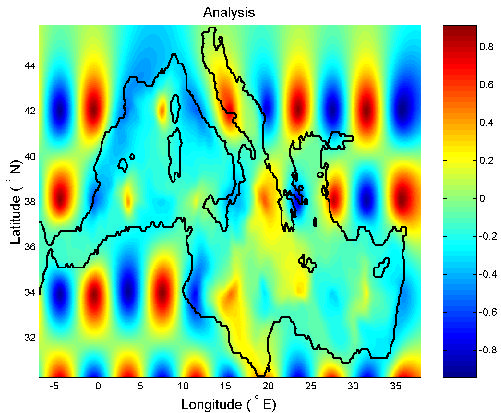
\includegraphics[width=.55\textwidth]{medregadv}
}\parbox{.4\textwidth}{
\caption{\diva with advection (on full grid, no direct topography, but indirect 
via advection).\label{fig:medsea_adv}}
}
\end{figure}


\begin{figure}[H]
\centering
\parbox{.6\textwidth}{
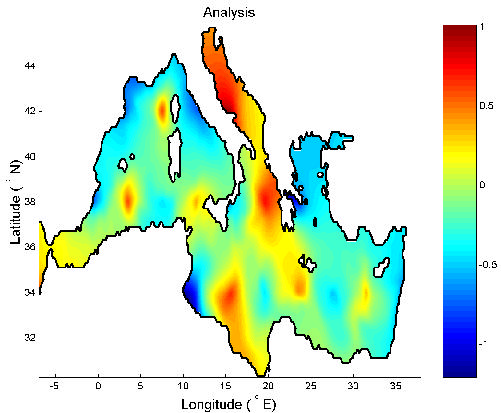
\includegraphics[width=.55\textwidth]{medregadvtopo}
}\parbox{.4\textwidth}{
\caption{\diva with topography and advection.}
}
\end{figure}


